\documentclass{beamer}
\usepackage{bibentry}
\bibliographystyle{plain}

\usepackage[utf8]{inputenc}
\usepackage[T1]{fontenc}
\usepackage{lmodern}
\usepackage[frenchb]{babel}
\usepackage{graphicx}

%\usetheme{Rochester}
\setbeamertemplate{navigation symbols}{}
\setbeamertemplate{footline}[frame number]
\newcommand\blfootnote[1]{%
  \begingroup
  \renewcommand\thefootnote{}\footnote{#1}%
  \addtocounter{footnote}{-1}%
  \endgroup}
\newcommand{\etal}{\emph{et al.}~}

\title{%
  Comité de Suivi de Thèse \\
  {\bf Analyse temporelle par vérification de modèles temporisés}}
\author{%
  Armel Mangean \\
  {\small\tt armel.mangean@irccyn.ec-nantes.fr}}
\institute{%
  École Centrale de Nantes \\
  IRCCyN, équipe Sytème Temps-Réel}
\date{Juin 2016}

\begin{document}

  \begin{frame}
    \small
    \nobibliography{refs.bib}
    \titlepage
  \end{frame}

  \section*{Avant-propos}
  \begin{frame}
    \frametitle{\secname}
    
    \vfill
    Sur le rapport et la soutenance de CST
    \begin{itemize}
      \item Réaliser dans l'urgence
      \begin{itemize}
        \item Soumission la semaine dernière
        \item {\color{gray} Engagements personnels}
          %% C'est peut-être déplacer mais c'est aussi un apprentisage
      \end{itemize}
      \item N'hésitez pas à poser des questions pendant la soutenance
    \end{itemize}
    \pause

    \vfill
    Sur la progression du travail
    \begin{itemize}
      \item Mêmes perspectives qu'en 2015
      \item Abandon de la première implémentation
      \item Réimplémentation (fonctionnelle)
    \end{itemize}

    \vfill
  \end{frame}

  \section*{Activités annexes}
  \begin{frame}
    \frametitle{\secname}
    
    \begin{block}{Formations doctorales}
      \begin{itemize}
        \item 36 heures de formation professionnelle\footnotemark[1]
        \item 25 heures de formation scientifique\footnotemark[1]
      \end{itemize}
    \end{block}

    \begin{block}{Enseignements}
      \begin{itemize}
        \item 77 heures de vacation\footnotemark[1]
        \item Étudiants de DUT Informatique
        \item Thématiques :
          \begin{itemize}
            \item Réseaux informatiques (base théorique)
            \item Réseaux informatiques (pratique)
            \item Architecture des ordinateurs
          \end{itemize}
      \end{itemize}
    \end{block}
    
    \footnotetext[1]{resp. 53, 40 et 114 heures sur 2014-2016}
  \end{frame}

  \begin{frame}
    \frametitle{Analyse temporelle par vérification de modèles temporisés}
    \tableofcontents
  \end{frame}

  % Deux points essentiels au calcul de WCET :
  %  - un modèle des composantes logicielles
  %  - un modèle des composantes matérielles
  \section{Rappel sur l'approche}
  \begin{frame}
    \frametitle{\secname}
    
    \begin{block}{Analyse temporelle}
      $\rightarrow$ Estimation de bornes supérieures sur les temps d'exécutions
    \end{block}

    \vfill
  %%   \begin{block}{Analyse par niveaux / \emph{bottom-up}}
  %%     \begin{itemize}
  %%       \item Estimation de WCET
  %%         \begin{itemize}
  %%           \item de blocs de base
  %%           \item de tâches (grâce au WCET de ses blocs de base)
  %%           \item du système (grâce au WCET de ses tâches)
  %%         \end{itemize}
  %%     \end{itemize}
  %%   \end{block}
  %% \end{frame}

  %% \begin{frame}
  %%   \frametitle{\secname}
    
    \begin{block}{Vérifications de modèles temporisés}
      $\rightarrow$ Vérification algorithmique de satisfaction d'une propriété
      temporelle par un modèle temporisé
    \end{block}
    
    \vfill        
    \begin{block}{Intérêt et problèmatique}
      \begin{itemize}
        \item Modèles exacts de systèmes complexes
        \item \alert{Explosion de l'espace d'état}
          \begin{itemize}
            \item Nécessité d'abstraire le modèle de programme
            \item Nécessité de spécialiser l'exploration de  l'espace d'état
          \end{itemize}
      \end{itemize}
    \end{block}
  \end{frame}

  % Bibilographie sur le permier point
  \section{Abstraction de CFG}
  \begin{frame}
    \frametitle{Analyse temporelle par vérification de modèles temporisés}
    \tableofcontents[currentsection]
  \end{frame}
  
  \subsection{Reconstruction de CFG}
  \begin{frame}
    \frametitle{\secname}
    \framesubtitle{\subsecname}

    \begin{block}{Graphe de flot de contrôle}
      $\rightarrow$ $(V,E,i)$ avec $V$ les blocs de base, $E \subset V \times V$
      les arcs du flot de contrôle et $i \in V$ le point d'entrée
    \end{block}

    \vfill
    \begin{block}{Reconstruction de CFG}
      \begin{itemize}
        \item Procédé
          \begin{itemize}
            \item À partir d'un fichier exécutable
            \item Reconstruction des blocs de base
            \item Reconstruction des chemins du flot de contrôle
          \end{itemize}
        \item \alert{Pas de branchement calculé}
        \item \alert{\emph{Inlining} des fonctions}
      \end{itemize}
    \end{block}
  \end{frame}

  \subsection{Abstraction de CFG}
  \begin{frame}
    \frametitle{\secname}
    \framesubtitle{\subsecname}

    % Comportement équivalent vis-à-vis d'un comportement spécifié
    % Suppression des instructions non concerné : réduction du modèle
    \begin{block}{\textit{Program Slicing}}
      $\rightarrow$ Calcul de l'ensemble des instructions affectant un
      sous-ensemble des variables du programme à un instant donné de son
      exécution
      \begin{itemize}
        \item Critère, tuple $C =~(l, v)$ avec
          \begin{itemize}
            \item $l$ un label
            \item $v$ un sous-ensemble des variables
          \end{itemize}
      \end{itemize}
    \end{block}

    \vfill
    \begin{block}{Interet pour l'abstraction de CFG}
      \begin{itemize}
        \item \emph{Slicing} sur l'ensemble des instructions de contrôle
        \item Abstraction de l'ensemble des autres instructions
        \item Contention de l'explosion de l'espace d'état
      \end{itemize}
    \end{block}
  \end{frame}

  \subsection*{Exemple de slicing}
  \begin{frame}
    \frametitle{\secname}
    \framesubtitle{\subsecname}
    
    \begin{figure}
      \centering
      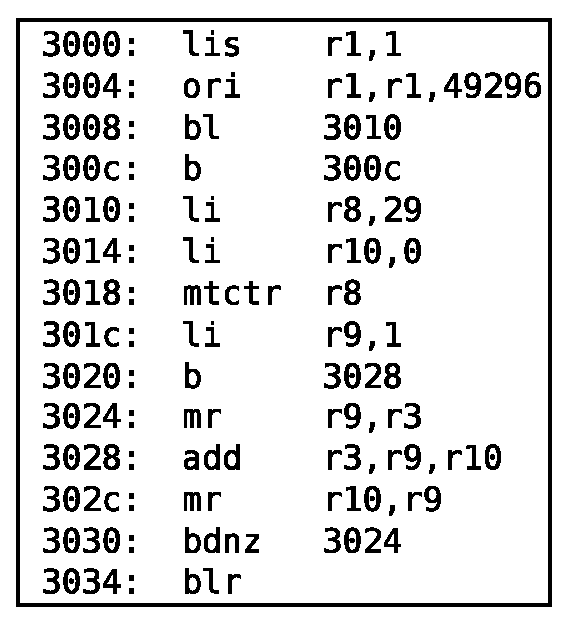
\includegraphics[scale=.5]{img/dump.eps}\hspace{1cm}
      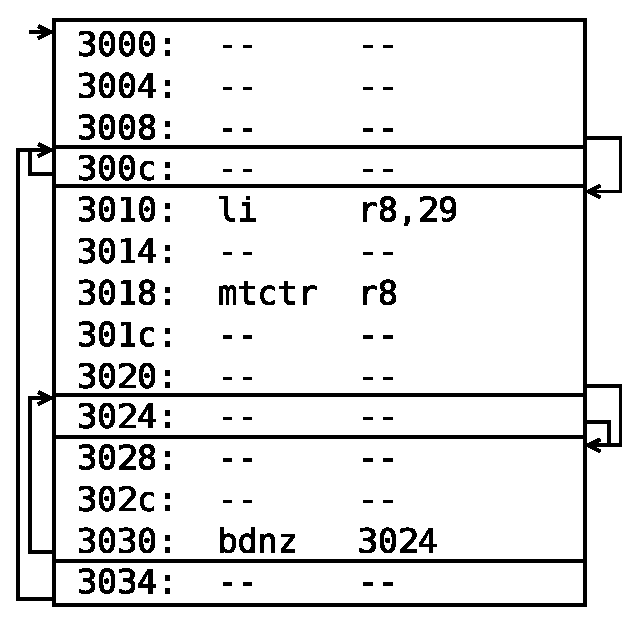
\includegraphics[scale=.5]{img/slice.eps}
      \caption{\texttt{fibcall-O2.elf}~;~$C =~(3030, \{ctr\})$}
    \end{figure}
  \end{frame}
  
  \begin{frame}
    \frametitle{\secname}
    %\framesubtitle{\subsecname}
    
    \begin{exampleblock}{Approches existantes}
      \tiny
      \begin{itemize}
        \item \bibentry{Wei81}
        \item \bibentry{Tip95}
        \item \bibentry{Agr94}
        \item \bibentry{CF97}
        \item \bibentry{KJL03}
      \end{itemize}
    \end{exampleblock}
  \end{frame}

  % Mise en oeuvre pratique sur le premier point
  \section{Développement d'un outil}
  \begin{frame}
    \frametitle{Analyse temporelle par vérification de modèles temporisés}
    \tableofcontents[currentsection]
  \end{frame}
  
  \subsection{Conception}
  \begin{frame}
    \frametitle{\secname}
    \framesubtitle{\subsecname}
    \small
    \begin{block}{\textsc{C++}}
      Langage de programmation impératif orienté objet \\
      \tiny
      \bibentry{Str86}
    \end{block}

    \begin{block}{\textsc{Lemon}}
      Bibliothèque (basée \emph{template}) optimisée de manipulation de graphes \\
      \tiny
      \bibentry{DJK11}
    \end{block}

    \begin{block}{\textsc{Harmless}}
      HADL et générateur de simulateurs \\
      Analyse sématique des fichiers exécutables \\
      \tiny
      \bibentry{KBB12}
    \end{block}
  \end{frame}

  \begin{frame}
    \frametitle{\secname}
    %\framesubtitle{\subsecname}
    
    \begin{block}{\textsc{Best}}
      $\rightarrow$ \emph{the Binary Executable Slicing Tool}
      \begin{itemize}
        \item Logiciel libre\footnotemark[1]
        \item Modularité vis-à-vis du jeu d'instruction
          \vspace{1em}
        \item Bancs d'essais
          \begin{itemize}
            \item \emph{benchmarks} WCET de Mälardalen
            \item Services du RTOS \textsc{Trampoline} (non publié)
          \end{itemize}
      \end{itemize}
    \end{block}

    \footnotetext[1]{Disponible à l'adresse \texttt{https://github.com/TrampolineRTOS/BEST}}
  \end{frame}
    
  \begin{frame}
    \frametitle{\secname}
    %\framesubtitle{\subsecname}
    
    \begin{figure}
      \centering
      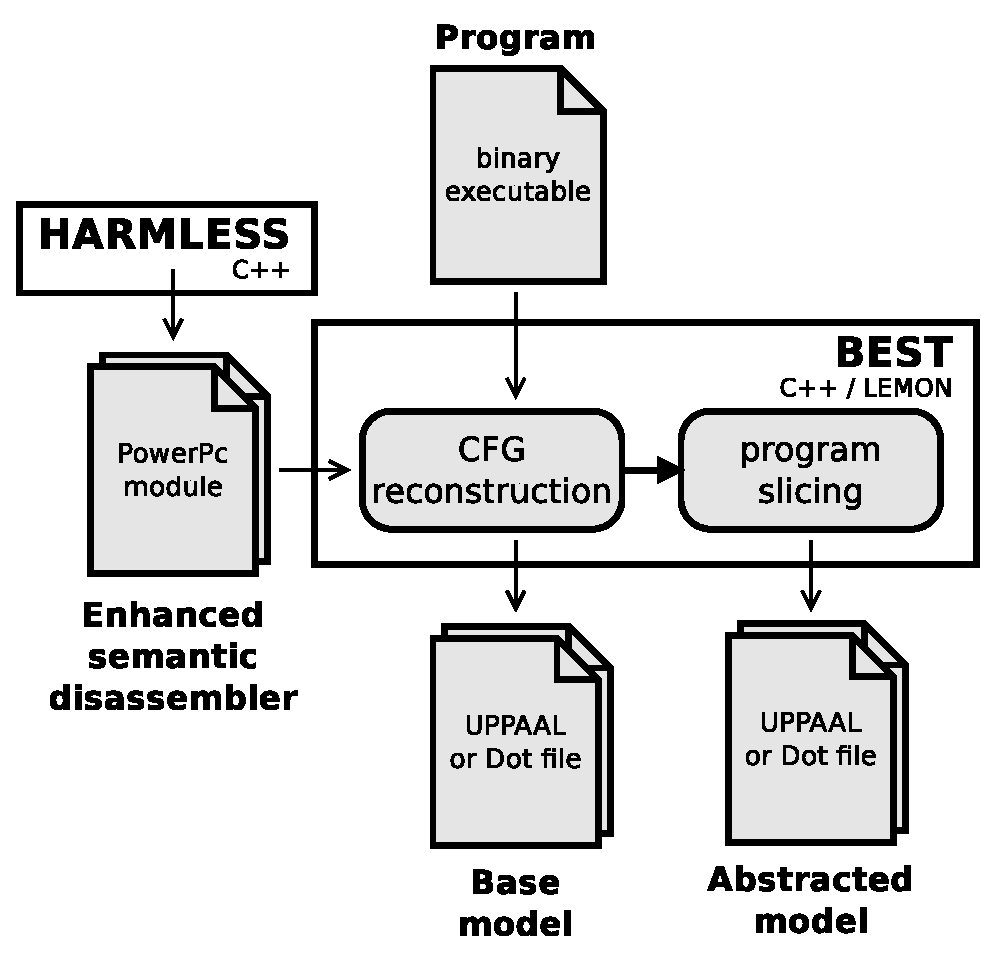
\includegraphics[scale=.4]{img/archi.eps}
      \caption{Architecture de l'outil}
    \end{figure}
  \end{frame}

  \section{Production scientifique}
  \begin{frame}
    \frametitle{\secname}
    \small
    
    \begin{block}{ETR'15}
      \begin{itemize}
        \item Écriture d'un article court et présentation d'un poster
      \end{itemize}
    \end{block}

    \begin{block}{JDoc'16}
      \begin{itemize}
        \item Formation doctorale obligatoire
        \item Écriture d'un article court et présentation d'un poster
      \end{itemize}
    \end{block}
    
    \begin{block}{SoC-SiP'16 (co-écriture)}
      \begin{itemize}
        \item Acceptation d'un \emph{Abstract} et présentation d'un poster
      \end{itemize}
    \end{block}
    
    \begin{block}{WCET'16 (co-écriture)}
      \begin{itemize}
        \item Soumission d'un article de \emph{workshop}
        \item Réponse le 7 juin $(?)$
      \end{itemize}
    \end{block}
  \end{frame}
  
  
  % Futur concerant le second point
  \section{Perspectives}
  \begin{frame}
    \frametitle{\secname}

    \vfill
    \begin{itemize}
      \item Poursuite du travail sur l'outil
        \begin{itemize}
          \item Gestion des cadres de piles
          \item Gestion de l'inter-procéduralité
          \item Exploitation des résultat avec \textsc{Trampoline}
        \end{itemize}
    \end{itemize}

    \vfill
    \begin{itemize}
      \item Modèlisation du matériel multi-c{\oe}ur
      \item Spécialisation de l'algorithme de vérification
    \end{itemize}
    
    \vfill
  \end{frame}
\end{document}
